%%%%%%%%%%%%%%%%%%%%%%%%%%%%%%%%%%%%%%%%%%%%%%%%%%%%%%%%%%%%%%%%%%%%%%%%%%%%%%%%
\chapter{Using Landslide}
%%%%%%%%%%%%%%%%%%%%%%%%%%%%%%%%%%%%%%%%%%%%%%%%%%%%%%%%%%%%%%%%%%%%%%%%%%%%%%%%
\label{sec:using}

In this chapter we discuss how to use Landslide with a kernel that meets 15-410's Pebbles specification. We list some design requirements that a Pebbles kernel must meet, document the instrumentation process and how to customise Landslide's search behaviour, and tell how to interpret Landslide's results.

In preparation for conducting the student user study (Section~\ref{sec:eval-studence}), we distributed a user guide roughly similar to this chapter.\footnote{
The user guide itself is available at \url{http://bblum.net/landslide-guide.pdf}, and at \url{http://www.contrib.andrew.cmu.edu/~bblum/landslide-guide.pdf}.}

%%%%%%%%%%%%%%%%%%%%%%%%%%%%%%%%%%%%%%%%%%%%%%%%%%%%%%%%%%%%%%%%%%%%%%%%%%%%%%%%
\section{Kernel Requirements}
\label{sec:using-requirements}

\subsection{Scheduler Functionality}
\label{sec:using-requirements-sched}

In order to cause desired preemptions, Landslide needs to assume that the core of the scheduler works. In short, this means that timer interrupts will trigger context switches, and that if a thread is ``runnable'', at any point where interrupts/preemption is enabled, a finite number of timer preemptions will eventually cause that thread to run.

For deadlock detection, if the kernel has mutexes which loop around a call to \texttt{yield} (or similar), they must be annotated as described in section~\ref{sec:using-annotations}. If mutexes explicitly deschedule blocking threads, no special annotations are needed.

Landslide does not support kernels that spin-wait anywhere, whether in mutexes or otherwise, especially when waiting for keyboard input or in \texttt{sleep}. Relatedly, the kernel must never run the idle loop when not truly idle, because Landslide uses this as a way of telling when all threads are wedged and/or when the test is done running.

\subsection{VM}

Landslide does not have much to do with the VM, but the kernel must direct-map most of kernel memory, including the heap, globals, and kernel thread stacks. Landslide needs this to read values out of memory and to identify memory conflicts.\footnote{
It would be simple to support more advanced virtual memory set-ups, in which the same virtual address has different physical memory mappings at different times, but this is not implemented.}

The kernel should also use LMM (the \texttt{malloc} package in the 15-410 base code) for dynamic allocation.

\subsection{System Calls}

In order to run with Landslide, the kernel must be able to boot up to the shell prompt\footnote{
In Pebbles, the bootup sequence is usually fairly simple, involving the init process spawning the shell.},
receive keyboard input to make the shell start a test case, and return to the shell prompt after the test case finishes. The kernel must have the following system calls implemented and working in at least a rudimentary way:
\texttt{fork}, \texttt{exec}, \texttt{vanish}, \texttt{wait}, \texttt{readline}.

The following system calls are exercised in some, but not all, of the test cases we distribute, so are helpful to have, but not necessary:
\texttt{thread\_fork}, \texttt{yield}.

Apart from the system calls which init and shell execute, the rest are irrelevant and do not need to be implemented to use Landslide on a Pebbles kernel.

%%%%%%%%%%%%%%%%%%%%%%%%%%%%%%%%%%%%%%%%%%%%%%%%%%%%%%%%%%%%%%%%%%%%%%%%%%%%%%%%
\section{Instrumenting Kernels with Landslide}
\label{sec:using-instrumenting}

Here we describe the interface by which Landslide understands the execution of the guest kernel. Landslide tries to be as design-agnostic as possible, after assuming that the kernel implements the Pebbles specification, but it still needs to know about the implementation of certain abstractions within the kernel.

\subsection{In-Kernel Annotations}
\label{sec:using-annotations}

\begin{figure}[h]
	\centering
	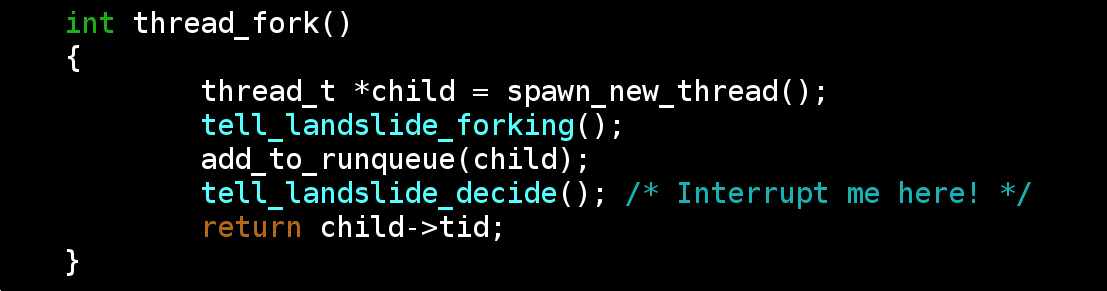
\includegraphics[width=\textwidth]{tell_landslide.png}
	\caption{Example annotated code. In theory, the use of \texttt{tell\_landslide\_decide()} in the place where a preemption needs to occur is not necessary for Landslide to know to preempt then; it is shown for the sake of demonstration.}
	\label{fig:tell-landslide}
\end{figure}

We provide a set of functions that the kernel needs to call at certain points during its execution to communicate what interesting events are happening. Figure~\ref{fig:tell-landslide} shows some example code annotated for Landslide.

\subsubsection{Important Note about Runqueues}
\label{sec:using-runqueue}
Landslide uses two of these annotations, \texttt{on\_rq()} and \texttt{off\_rq()}, for tracking the state of the scheduler's runqueue at each point during execution.
Note that this refers to the {\em actual runqueue data structure}, which does not necessarily correspond to the abstract ``set of all runnable threads'', depending on whether or not the kernel keeps the current thread on the runqueue or off of it.

If the kernel does not keep the currently-running thread on the runqueue, the user must also use \texttt{kern\_current\_extra\_runnable} (Section~\ref{sec:using-student-c}).

\subsubsection{Required Annotations}
\begin{itemize}
	\small
	\item \texttt{tell\_landslide\_thread\_switch(int new\_tid)} - Call this in the context switcher, when a new thread is switched to.
	\item \texttt{tell\_landslide\_sched\_init\_done()} - Call this when the scheduler is done being initialized. Until this is called, Landslide will ignore all other annotations.
	\item \texttt{tell\_landslide\_forking()} - Call this when a new thread is being forked.
		(Hint: call it twice, once in \texttt{fork} and once in \texttt{thread\_fork}.)

		Call it ``just before'' the action which makes the new thread runnable - whether the kernel just adds it to the runqueue (in which case the next annotation called would be \texttt{thread\_on\_rq}) or begins running it immediately (in which case \texttt{thread\_switch}); Landslide handles both cases.
	\item \texttt{tell\_landslide\_vanishing()} - Call this when a thread is about to go away.
		Call it ``just before'' the relevant context switch; i.e., the one that should never return.
	\item \texttt{tell\_landslide\_sleeping()} - Call this when a thread is about to go to sleep (that's \texttt{sleep()} the system call).
		Call it ``just before'' the relevant context switch; i.e., the one that won't return for as long as the thread requested to sleep.
	\item \texttt{tell\_landslide\_thread\_on\_rq(int tid)} - Call this when a thread is about to be added to the runqueue.
		(Make sure this call is done within whatever protection is also used for the runqueue modification itself.)
	\item \texttt{tell\_landslide\_thread\_off\_rq(int tid)} - Call this when a thread is about to be removed from the runqueue. (Same protection clause as above applies.)
	\item Mutex annotations - These are only necessary if the kernel uses mutexes that leave blocked threads on the runqueue, rather than explicitly descheduling them.
	\begin{itemize}
		\item \texttt{tell\_landslide\_mutex\_locking(void *mutex\_addr)} - Call this when a thread is about to start locking a mutex. Landslide needs the mutex address for deadlock detection, to track which mutex each thread is blocked on.
		\item \texttt{tell\_landslide\_mutex\_locking\_done()} - Call this when a thread finishes locking a mutex (and now owns it).
		\item \texttt{tell\_landslide\_mutex\_unlocking(void *mutex\_addr)} - Call this when a thread is about to start unlocking a mutex.
		\item \texttt{tell\_landslide\_mutex\_unlocking\_done()} - Call this when a thread finishes unlocking a mutex (and no longer owns it).
		\item \texttt{tell\_landslide\_mutex\_blocking(int owner\_tid)} - Call this when a thread is contending on a locked mutex, and hence is no longer logically ``runnable'' yet still on the runqueue. Landslide needs to know who owns the mutex for deadlock detection.
	\end{itemize}
\end{itemize}

\subsubsection{Optional Annotations}
\begin{itemize}
	\small
	\item \texttt{tell\_landslide\_decide()} - Call this to define additional decision points. See section~\ref{sec:using-decision}.
	\item \texttt{assert()} or \texttt{panic()} - You should be using these already, but they are extra useful in Landslide.
		The more important invariants for which a kernel has \texttt{assert}s, the more likely Landslide is to find bugs that would trigger them - otherwise, even if they do happen, Landslide might never know (just like in conventional stress testing).
\end{itemize}

\subsection{Configuration File}
\label{sec:using-config-landslide}

There is also a config file the user needs to fill out, called \texttt{config.landslide}. Some of the fields are required information, and some are tweaks that change the way Landslide behaves. We omit discussion of the required fields, and explain the optimisations and behaviour tweaks that Landslide supports in Section~\ref{sec:using-search}.

\subsection{Instrumenting Within Landslide}
\label{sec:using-student-c}

There are two functions that the user needs to implement in Landslide itself, in a file called \texttt{student.c}, to express certain kernel designs that might be more complicated than a simple true/false condition or integer.

\begin{itemize}
	\small
        \item \texttt{bool kern\_current\_extra\_runnable(conf\_object\_t *cpu)} - See Section~\ref{sec:using-runqueue}. This says whether the current thread is ``logically runnable'' despite not being on the runqueue itself (that is, \texttt{tell\_landslide\_on\_rq} won't have been called for it).
        \item \texttt{bool kern\_ready\_for\_timer\_interrupt(conf\_object\_t *cpu)} - This function can be used to express when the scheduler is ``locked'' in a way not involving disabled interrupts. Landslide will avoid trying to preempt the kernel whenever this is false.
\end{itemize}

%%%%%%%%%%%%%%%%%%%%%%%%%%%%%%%%%%%%%%%%%%%%%%%%%%%%%%%%%%%%%%%%%%%%%%%%%%%%%%%%
\section{Configuring Landslide's Behaviour}
\label{sec:using-customise}
\subsection{Decision Points}
\label{sec:using-decision}

Getting a good set of decision points is important to being able both to explore reasonably quickly and to produce meaningful interleavings that are likely to find bugs. After getting Landslide working with the default set of decision points (voluntary reschedules only), the next step is to add some more. We list here the general steps in this process.

\begin{itemize}
        \item Use \texttt{tell\_landslide\_decide()} to indicate decision points.\footnote{
	We recommend at the start of \texttt{mutex\_lock} and at the end of \texttt{mutex\_unlock}, though it is also important to use one's own intuition, depending on what system call(s) are being tested.}
        \item Use \texttt{sched\_func} and \texttt{ignore\_sym} to make Landslide ignore global memory accesses, to enable better pruning.
        \item Use \texttt{DECISION\_INFO\_ONLY} to examine the set of choice points, and figure out which ones are irrelevant.
        \item Use \texttt{within\_func} and \texttt{without\_func} to make Landslide only use relevant decision points.
\end{itemize}

\subsection{Search Parameters}
\label{sec:using-search}

Landslide's configuration file supports several options for changing the way it explores the decision tree.

\subsubsection{Optimizations}

These configuration options help Landslide identify potentially-conflicting shared memory accesses that it should ignore (Section~\ref{sec:por-independence}).

\begin{itemize}
	\small
	\item \texttt{sched\_func} - When functions that make up the kernel's scheduler are identified, Landslide knows to ignore shared memory accesses from them. Accesses to scheduler data structures happen during {\em every} transition, so ignoring these is necessary for achieving any reduction at all.
	\item \texttt{ignore\_sym} - The user may wish to ignore memory accesses from other global data structures as well. For example, ignoring a mutex which is locked very frequently, but irrelevant to the actual test case, will result in an independence relation that better reflects what is actually being tested for.
	\item \texttt{within\_function} - If the user configures decision points to happen in common code paths, such as \texttt{mutex\_lock}, it will likely generate more branching than needed.\footnote{
For example, if testing \texttt{vanish}, there's no need to branch on a \texttt{mutex\_lock} in \texttt{exec}.}
This configuration option allows the user to whitelist functions so that Landslide will only decide if the current thread is ``within'' one of those functions.
	\item \texttt{without\_function} - Similar to above, but a blacklist. These two can be used together; later invocations take precedence over earlier ones.
\end{itemize}

\subsubsection{Behaviour Tweaks}
\begin{itemize}
	\small
	\item \texttt{EXPLORE\_BACKWARDS} - In which order to explore the branches? Backwards means with more preemptions first; forwards means tending to let the current thread keep running more often. Backwards tends to find bugs more quickly, but produces longer decision traces. (Section~\ref{sec:future-backwards})
	\item \texttt{DECISION\_INFO\_ONLY} - This option makes Landslide stop after one branch, and output the list of decision points it identified using the current config. Useful to see all decision points, and tweak settings to get rid of frivolous ones.
\end{itemize}

%%%%%%%%%%%%%%%%%%%%%%%%%%%%%%%%%%%%%%%%%%%%%%%%%%%%%%%%%%%%%%%%%%%%%%%%%%%%%%%%
\section{Test Cases}
\label{sec:using-tests}

We ship Landslide with a suite of small test cases designed to expose several common races that students frequently encounter during 15-410 Project 3. We list their code in Appendix~\ref{sec:test-code}.

\begin{itemize}
        \item \texttt{vanish\_vanish} - Tests when a parent and child process \texttt{vanish()} simultaneously.
        \item \texttt{double\_wait} - Tests interactions of multiple waiters on a single child.
        \item \texttt{double\_thread\_fork} - Tests for interactions of multiple threads in one process vanishing.
        \item \texttt{yield\_vanish} - Tests for interactions between \texttt{yield()} and \texttt{vanish()}.
\end{itemize}

\subsection{Landslide-Friendly Test Characteristics}
\label{sec:using-landslide-friendly-tests}

It is important to note why all of these test cases are ``Landslide-friendly'': they all perform very little work on a single run, enabling Landslide to completely explore the state-space. They also run several, but not too many, threads at once, producing potentially interesting interleavings.
